\renewcommand{\thechapter}{\roman{chapter}}
\setcounter{chapter}{1}
\setcounter{figure}{0}

\unchapter{Introduction}
\label{chap:introduction}
% \addcontentsline{toc}{chapter}{Introduction}
La peau est le plus important organe en surface du corps humain et ses lésions sont nombreuses~: des plus anodines (communément appelées lésions bénignes), aux plus graves (dites lésions malignes) comprenant divers cancers aux répercussions les plus dramatiques.\par

La plupart des lésions malignes rencontrées sont d’origine cancéreuse, issues d’une division ou d’une mutation anormale de cellules de la peau et, résultent pour la plupart d’une exposition aux \gls{uv}, principal facteur de risque. D’autres facteurs tels que le tabagisme, les virus, des prédispositions génétiques ou encore l’utilisation de médicaments immunosuppresseurs (à la suite d'une transplantation par exemple) favorisent leur apparition. Afin de limiter l’incidence de ces lésions, de nombreuses campagnes de prévention sont menées, intégrant sensibilisation et actions de prévention dans le but d’augmenter le confort de vie futur des individus, notamment au sein des pays les plus touchés.\par

Ces campagnes de sensibilisation à la prévention, bien que souvent sous des formes traditionnelles tel que des prospectus ou spots publicitaires, peuvent être de natures diverses. Nous pouvons citer à titre d’exemple, la mise en place de formations de prévention dès le plus jeune âge au sein des structures scolaires aux États-Unis d’Amérique, ou à l’opposé la multiplication des supports de communication avec, par exemple, l’utilisation de sachets de sucres au Portugal \cite{Correia2017,Guy2016}.\par 

\begin{table}[H]
    \begin{tabular}{lll|lll}
    \textbf{Cancer}                     & \textbf{Incidence}& \textbf{Décès}& Prostate cancer                  & 1618               & 366           \\
    All cancers                         & 17481             & 8713          &  Testicular cancer               & 72                 & 9             \\
    Lip and oral cavity                 & 410               & 146           &  Kidney cancer                   & 425                & 137           \\
    Nasopharynx cancer                  & 123               & 63            &  Bladder cancer                  & 541                & 188           \\
    Other pharynx                       & 161               & 64            &  Système nerveux cancer          & 321                & 229           \\
    Esophageal cancer                   & 1313              & 891           &  Thyroid cancer                  & 334                & 32            \\
    Colon and rectum cancer             & 1653              & 832           &  Mesothelioma                    & 37                 & 32            \\
    Gallblader and biliary tract cancer & 188               & 140           &  Hodgkin lymphoma                & 78                 & 24            \\
    Pancreatic cancer                   & 426               & 412           &  Non Hodgkin lymphoma            & 666                & 231           \\
    Larynx cancer                       & 238               & 106           &  Multiple melyoma                & 154                & 101           \\
    Tracheal, bronchus and lung cancer  & 2019              & 1722          &  Leukemia                        & 606                & 353           \\
    Malignant skin melanoma             & 352               & 60            &  Acute lymphoid leukemia         & 161                & 110           \\
    Breast cancer                       & 2422              & 534           &  Chronic lymphoid leukemia       & 191                & 61            \\
    Cervical cancer                     & 526               & 239           &  Acute myeloid leukemia          & 190                & 147           \\
    Uterine cancer                      & 455               & 90            &  Chronic myeloid leukemia        & 64                 & 35            \\
    Ovarian cancer                      & 251               & 161           &  Other neoplasms                 & 756                & 372           \\
    \end{tabular}    
    \caption{Statistiques mondiales d’incidence et mortalité par type de cancers~\cite{Karimkhani2017}. Les chiffres indiqués dans le tableau (incidence et décès) sont exprimés en milliers.}
    \label{tab:introduction_cancer_incidence}
\end{table}\par

Néanmoins, ces actions tendent aujourd’hui à dépasser la prévention. En effet, certains articles essaient de montrer l’importance d’une auto-surveillance régulière des individus au travers de gestes simples, dans le cadre de la détection de mélanome, permettant une prise en charge de la pathologie dans un meilleur délai. Dans ce même objectif, nous pouvons également mentionner l’accroissement du nombre de campagnes de dépistage mises en place par les gouvernements \cite{Friedman1985}.\par

Malgré ces démarches, le taux d’apparition de ces cancers ne cesse d’augmenter dans le monde. De nos jours, l'\gls{who} dénombre~:
\begin{itemize}
    \item entre 2 et 3 millions de cancers de la peau autres que le mélanome par an
    \item environ 132 000 cancers de type mélanome par an.
\end{itemize} La table \Cref{tab:introduction_cancer_incidence} recense les divers types de forme cancéreuses incidence et mortalité associé pour l'année 2015. \par

D'un point de vue financier, les soins générés par les pathologies de la peau (toutes confondues) se chiffrent annuellement à 8 milliards de dollars aux États-Unis \cite{Farberg2017a}.\par

Pour la France, ce n’est pas moins de 5 100 nouveaux cas par an estimés de mélanome chez la femme et 4 680 chez l’homme, soit respectivement la 6ème et 8ème cause de cancer. Cette pathologie provoque environ 1 500 décès par an, genres confondus \cite{Thuret2012}.\par

Notre sujet « \titleref » s’inscrit dans cette thématique, en tentant d’apporter des outils permettant d’aider le praticien dans sa prise de décision.\par

Cette thèse répond donc en premier lieu à un besoin sociétal, d'autant plus de la baisse constante du nombre de dermatologues en France depuis 2010, visible en \Cref{fig:number_dermatologists}.
\begin{figure}[H]
    \centering
    \includegraphics[width=\linewidth]{contents/i_introduction/resources/evolution_dermatologists.pdf}
    \caption{Évolution du nombre de dermatologues en France entre les années 1999 et 2017 \textsuperscript{\ref{footnote:number_dermatologists}}.}
    \label{fig:number_dermatologists}
\end{figure}\par
\addtocounter{footnote}{1}
\footnotetext[\thefootnote]{Source image~: Graphique généré à partir de données en provenance du site du  \href{http://www.data.drees.sante.gouv.fr/}{gouvernement} sur la santé. \label{footnote:number_dermatologists}}

Néanmoins, cette thématique ne demeure pas moins intéressante d’un point de vue scientifique. En effet, les 20 dernières années ont été portées par une forte tendance sur le sujet comme le démontre la \Cref{fig:evolution_publications}. Cette tendance est régie par plusieurs facteurs~:
\begin{itemize}
    \item Le besoin sociétal de la thématique, et l'intérêt porté par les industriels
    \item Le phénomène "machine learning", et ses récentes avancées (notamment avec l'apprentissage profond)
    \item Le "challenge" apporté par cette thématique, que nous développerons.
\end{itemize}\par

Ce travail tente d'apporter de nouveaux éléments de résolution, par l’apport notamment d’une dimension de multi modalité encore peu exploitée dans cette branche. 
\begin{figure}[H]
    \centering
    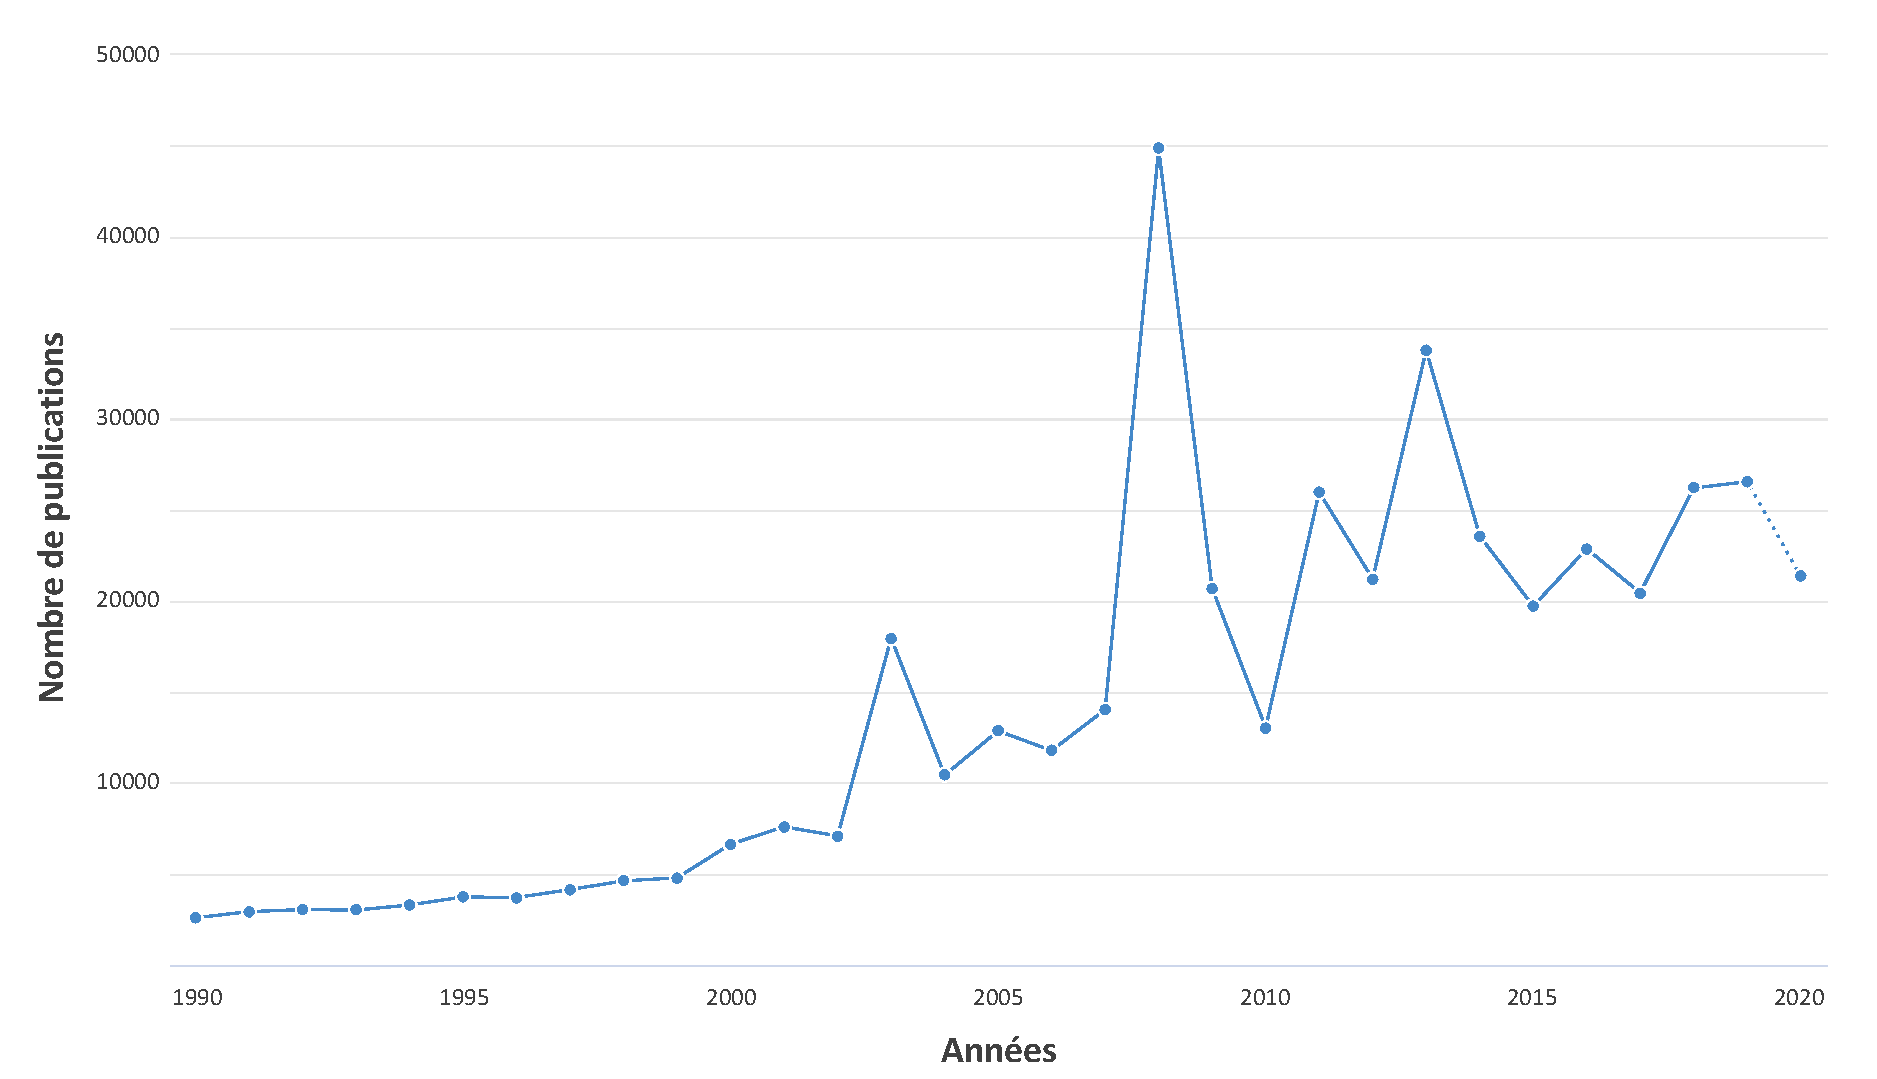
\includegraphics[width=\linewidth]{contents/i_introduction/resources/evolution_publications.pdf}
    \caption{Évolution de la recherche autour des termes "skin lesion computer diagnosis" durant ces 20 dernières années \textsuperscript{\ref{footnote:evolution_publications}}.}
    \label{fig:evolution_publications}
\end{figure}\par
\addtocounter{footnote}{1}
\footnotetext[\thefootnote]{Source image~: Graphique généré à partir de données en provenance du moteur de recherche \href{https://scholar.google.fr/}{Google Scholar.} \label{footnote:evolution_publications}}

Ce travail s'inscrit dans une démarche d'aide au diagnostic des lésions de la peau et particulièrement des pathologies de \gls{lm} et \gls{lmm}. De nombreux travaux se sont portés sur l'aide à la détection par ordinateur de lésions de la peau à partir d'une modalité unique d'imagerie. Néanmoins, peu d'entre eux s'intéressent à une démarche multimodale de cette thématique, soit par non-considération de cette application, soit par manque ou insuffisance de données à leur disposition.\par

La matière première mise à notre disposition permet une orientation de nos travaux dans le sens de la multimodalité. En effet, l'une des problématique majeure aujourd'hui en dermatologie est ce que les médecins qualifient de zone d'indécision, également appelée \textit{zone grise}. Il s'agit d'une catégorie de cas cliniques pour lesquels le médecin n'a pas à un instant $t$ suffisamment d'information ou de connaissances pour prendre une décision. Ces cas nécessitent souvent une prise en charge plus importante, avec l'aide d'autres spécialistes ou encore avec notamment de nouveaux examens plus spécifiques.\par

La finalité de ce travail est de proposer diverses techniques et outils permettant une aide à la décision dans la gestion de cette zone grise, et ainsi améliorer la prise en charge clinique en service de dermatologie. Ainsi, nous proposons un schéma macroscopique de cet objectif sur la \Cref{fig:scheme_reduce_indecision}.\par

\begin{figure}[H]
    \centering
    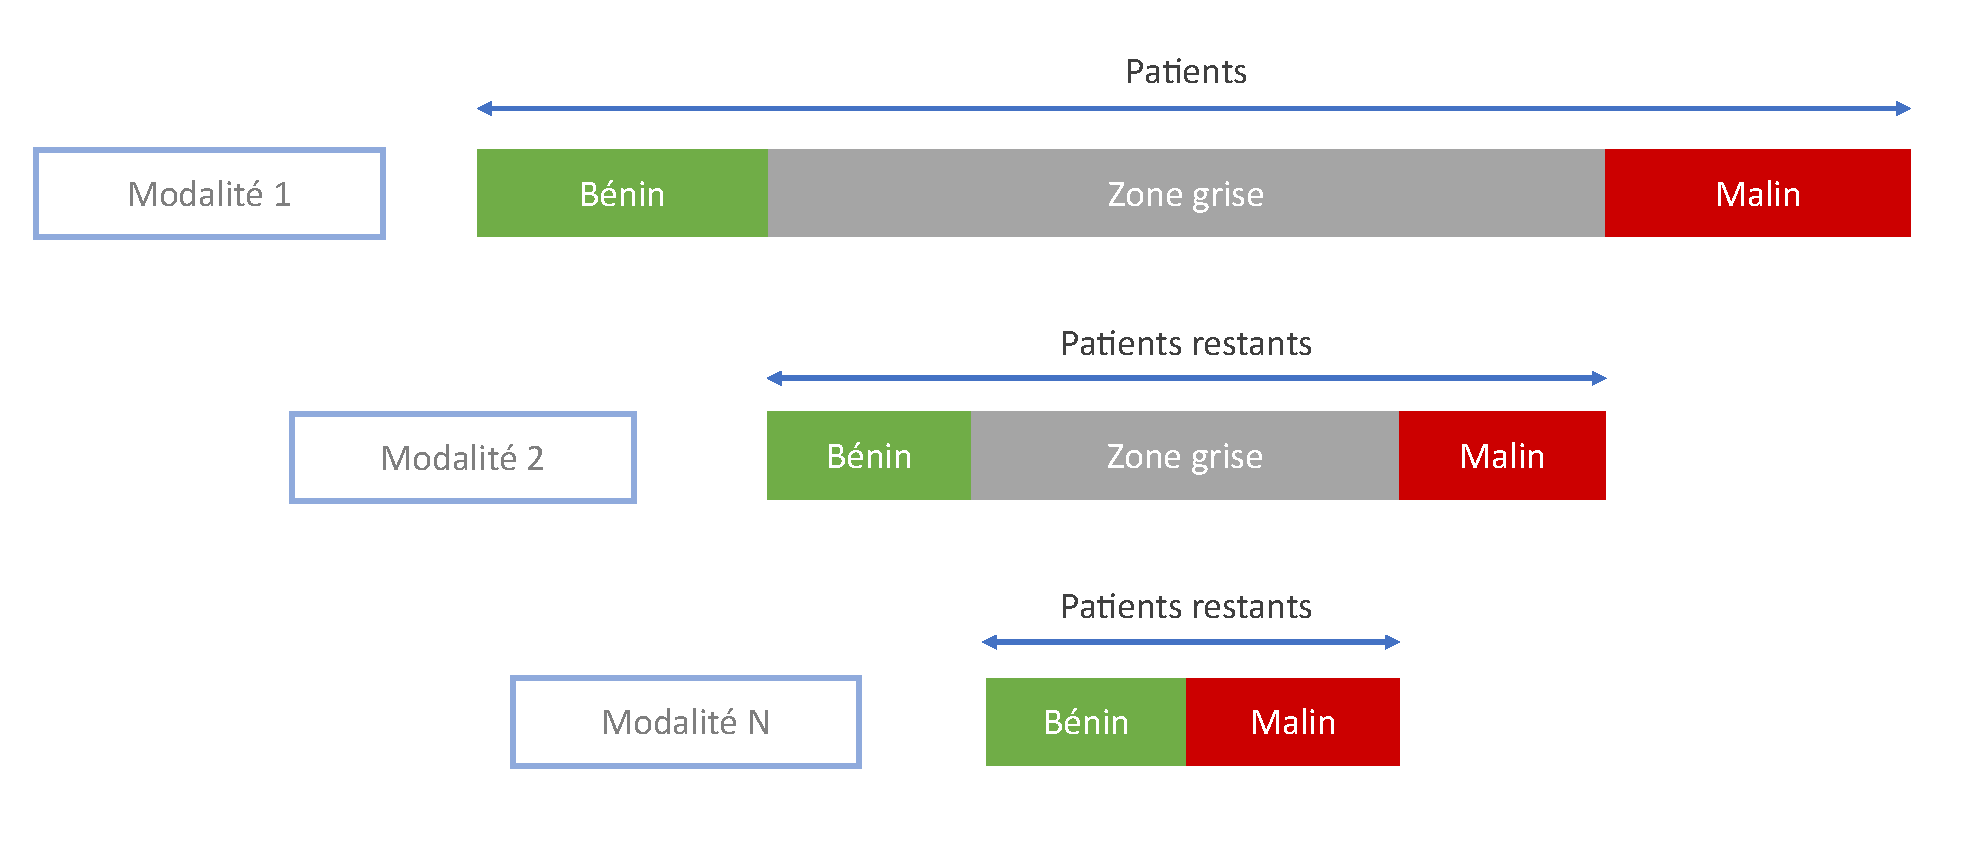
\includegraphics[width=\linewidth]{contents/i_introduction/resources/scheme_reduce_indecision.pdf}
    \caption{Représentation du processus de réduction de l'indécision du médecin ou \textit{zone grise}. L'objectif de ce travail consiste à réduire cette indécision des divers cas d'études en notre possession, par l'ajout de modalités d'imagerie en s'inspirant du processus cognitif des dermatologues.}
    \label{fig:scheme_reduce_indecision}
\end{figure}\par

Dans ce schéma idéal représenté sur la \Cref{fig:scheme_reduce_indecision}, les patients jugé avec une certaine certitude comme "bénin" ou "malin", seront exclus des procédures suivantes. Seuls les patients encore présents dans cette "zone grise" seront pris en charge pour des examens supplémentaires, par lesquels nous réitérons ce processus.\par 

A cette fin, nous mobiliserons des connaissances en provenance de divers champs d'applications propre~:
\begin{inlinerate}
    \item à la peau d'un point de vue médical, 
    \item aux modalités permettant l'observation des tissus,
    \item et à l'intelligence artificielle.
\end{inlinerate} Cette complémentarité est représentée sous forme de schéma macroscopique sur la \Cref{fig:scheme_our_work}.\par

\begin{figure}[H]
    \centering
    \includegraphics[width=0.8\linewidth]{contents/i_introduction/resources/scheme_our_work.pdf}
    \caption{Représentation macroscopique des domaines impliqués de cette thématique de recherche. Notre travail se retrouve ainsi aux confluents de connaissances de la peau, des modalités d'imagerie permettant son acquisition et des domaines de l'intelligence artificielle.}
    \label{fig:scheme_our_work}
\end{figure}\par

Dans un premier temps, nous aborderons le contexte de cette étude dans la \Cref{part:contexte}. Ainsi, nous débuterons au sein du \Cref{chap:chapter_1} par une présentation de la peau, l'organe majeur de cette étude. Puis, nous procéderons dans le \Cref{chap:chapter_2} à une mise en évidence des principes d'interaction entre la peau et la lumière, avant de présenter les techniques de visualisation mises à disposition des médecins. Pour finir cette partie, le \Cref{chap:chapter_3} met à la disposition du lecteur l'ensemble des connaissances d'intelligence artificielle sollicitées dans ce manuscrit.\par

Dans un second temps, nous nous consacrerons à l'aide de la \Cref{part:microscopy} au traitement de la modalité \gls{rcm}, qui met à notre disposition plusieurs images par lésions. A cet effet, nous débuterons par le traitement des images de cette modalité dans un \Cref{chap:chapter_4} dédié à la classification de ces images. Nous étendrons ces travaux dans le \Cref{chap:chapter_5}. Puis, nous terminerons l'analyse de cette modalité dans un \Cref{chap:chapter_6} dédié à la prise de décision au niveau d'une lésion.\par

Dans un dernier temps, nous nous consacrerons à la finalité de ce travail, celui de la multimodalité, par la \Cref{part:multimodal}. Le \Cref{chap:chapter_7} reprendra les travaux des autres modalités en notre possession ainsi que les conclusions de la \gls{rcm} et mettra en avant des méthodes d'agrégation de l'information.\par